\documentclass[11pt,letterpaper,twoside]{article}
\usepackage[english]{babel}
\usepackage{amssymb,amsmath}
\usepackage{fancyhdr}
\usepackage{graphicx}
\usepackage{wrapfig}

 \oddsidemargin  0in \evensidemargin 0in
 \topmargin   -0.25in \headheight 0.25in \headsep 0.25in
 \textwidth   6.5in \textheight 8.75in \marginparsep 0pt \marginparwidth 0pt
 \parskip 1ex  \parindent 0ex \footskip 20pt

\newfont{\bssten}{cmssbx10}
\newfont{\bssnine}{cmssbx10 scaled 900}

%%%%%%%%%%%%%%%%%%%%%%%
\newcommand{\whatizit}{Lecture 15: Point Estimates and Sampling Variability}
%%%%%%%%%%%%%%%%%%%%%%%


\pagestyle{fancy}  
\fancyhead{\bssnine STOR 155,  \whatizit}
\fancyhead[RE]{} \fancyhead[LO]{}
\fancyhead[LE]{\bssnine \thepage} \fancyhead[RO]{\bssnine \thepage}
\lfoot{} \cfoot{} \rfoot{}   


\newcommand{\var}{\mathrm{Var}}



\begin{document}



\thispagestyle{empty} \vspace*{-0.75in}

{\bssten STOR 155: Introduction to Data Models and Inference \hfill June 7, 2024 \\
Prof. Will Lassiter  \hfill Page 1 of \pageref{totalpag}}
\vspace{10pt}
\begin{center} {{\Large \bf \whatizit}} \end{center}

Terminology: Parameter, Statistic, Point Estimate \vspace{220pt}


{\bf Sampling Variability} \vspace{6pt}

Example: Heights of men at UNC

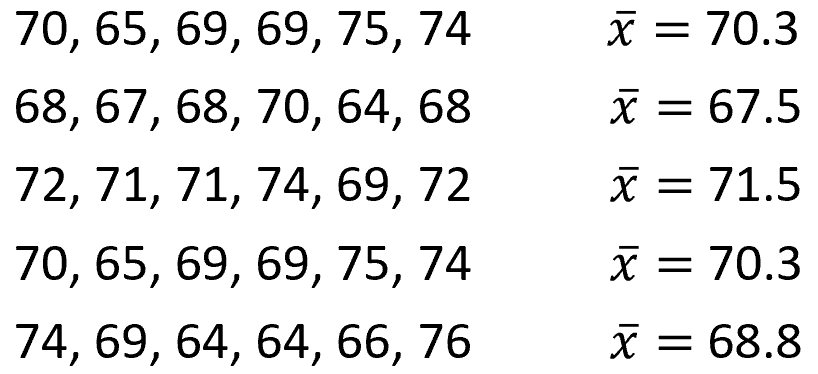
\includegraphics[scale=0.7]{images/heights.png}\hspace{20pt}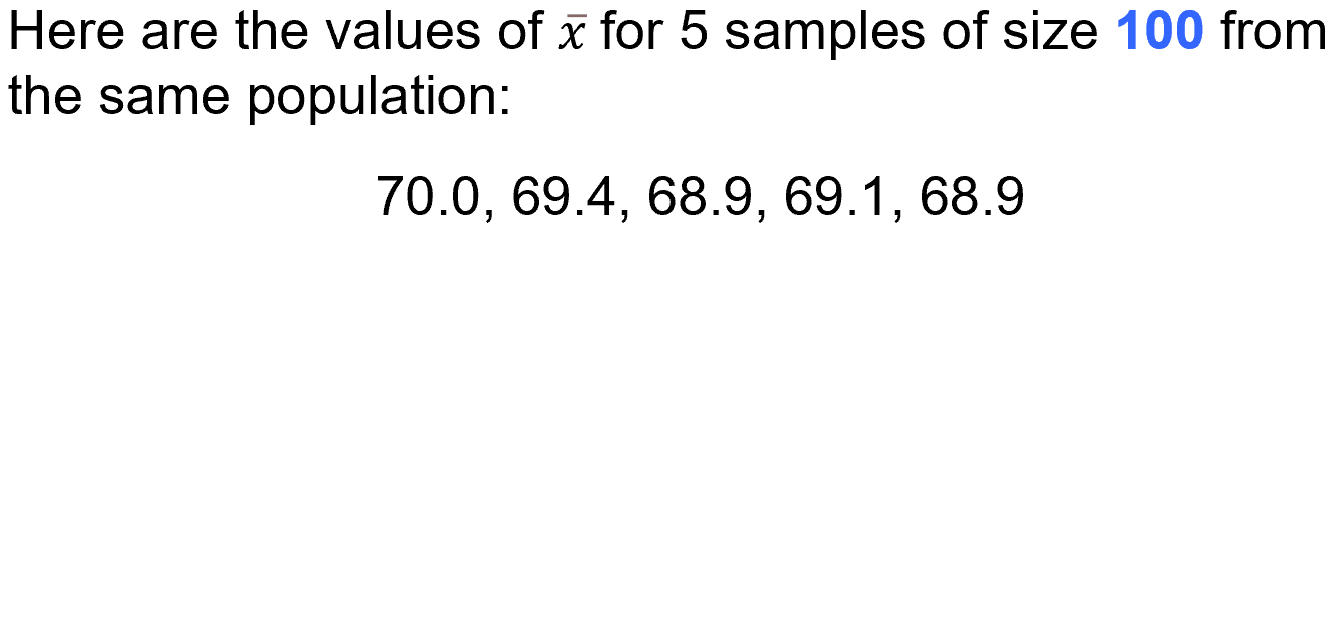
\includegraphics[scale=0.45]{images/heights2.png} \vspace{30pt}

\begin{center}
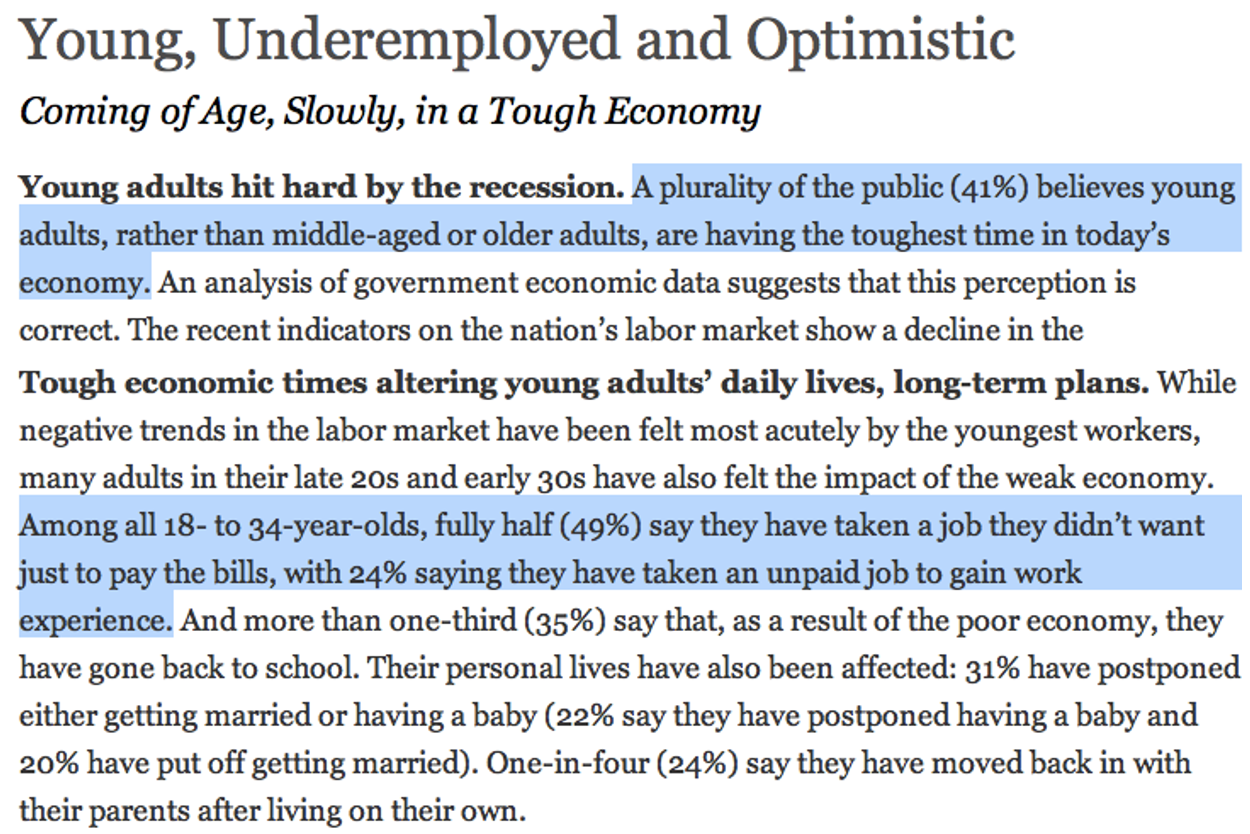
\includegraphics[scale=0.5]{images/pew1.png}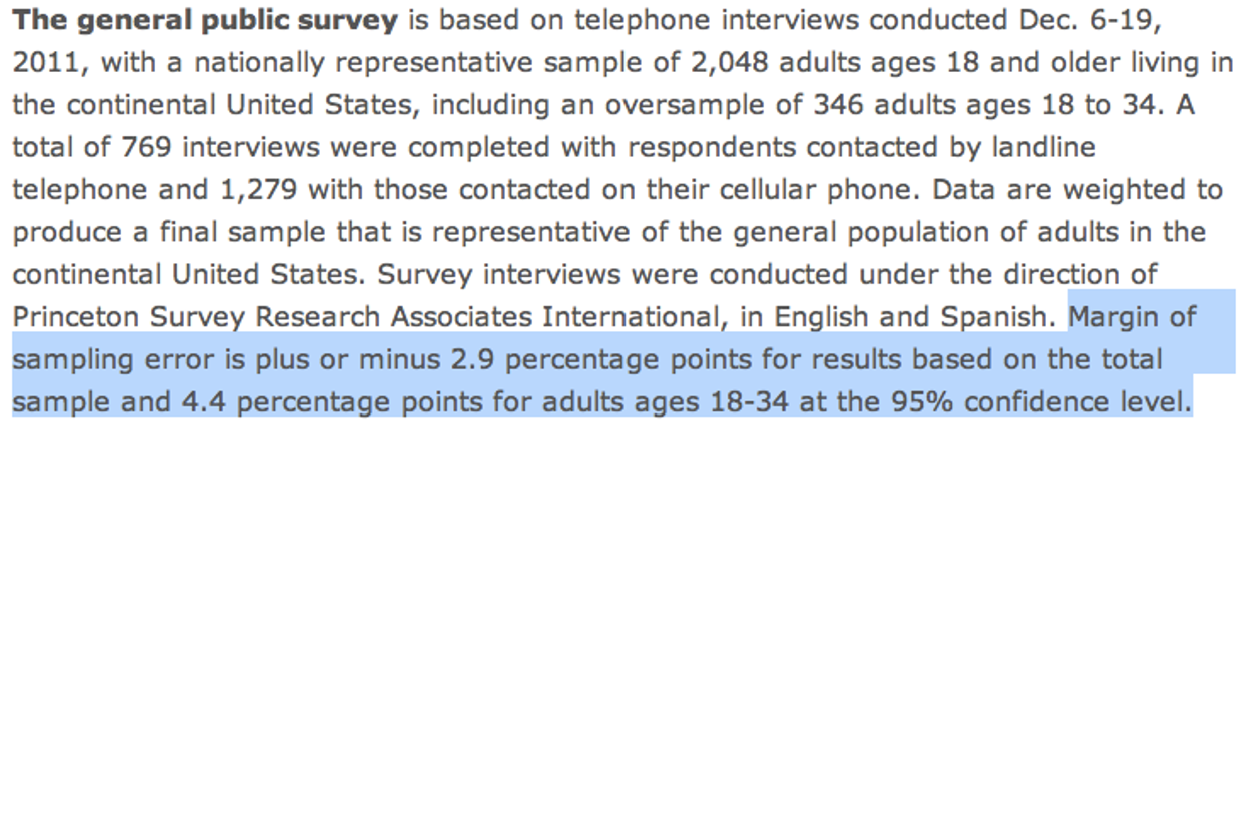
\includegraphics[scale=0.5]{images/pew2.png}
\end{center}

\newpage

Example: Suppose the proportion of all American adults who support the expansion of solar energy is $p = 0.88$, but we don't have access to the population of all American adults (a quite likely scenario) and thus can't know this true value of $p$. 

If we are interested in estimating $p$, a reasonable approach might be: \vspace{120pt}

\begin{center}
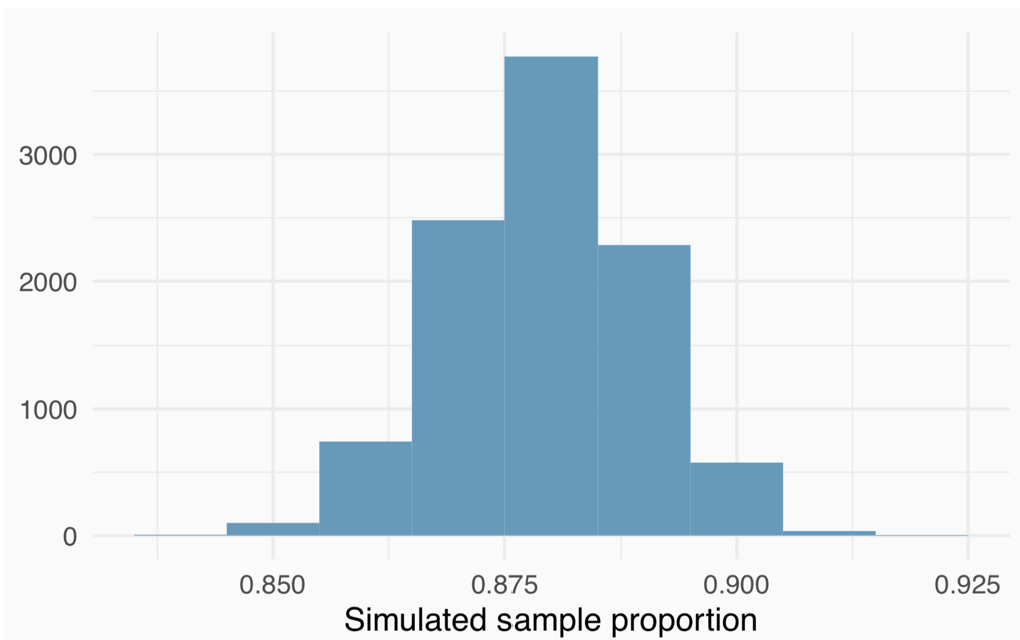
\includegraphics[scale=0.8]{images/sampling.png}
\end{center}

We will never actually observe a {\bf sampling distribution} like this one, but the {\bf Central Limit Theorem} describes its shape.

\newpage

Derivation of the sampling distribution for a sample proportion $\hat{p}$ \vspace{120pt}

Necessary conditions for CLT to apply:

\begin{itemize}

\item Independent Observations \vspace{100pt}

\item Adequate Sample Size \vspace{100pt}

\end{itemize}

Example:  Randomly sample $n = 2500$ American adults and ask whether they like ``The Office".  2400 respond ``Yes" and 100 respond ``No". \vspace{120pt}

If the true proportion $p$ of American adults who like ``The Office" was 0.9, with what probability would we obtain a random sample of 2500 adults with at least 2400 who like the show?

\newpage

More on CLT conditions:

\begin{itemize}

\item When either $np$ or $n(1-p)$ is small, the sampling distribution is more discrete and more skewed. The larger both $np$ and $n(1-p)$ are, the more normal the distribution looks.

\item When $np$ and $n(1-p)$ are both very large, the discreteness of the sampling distribution is hardly evident, and the distribution looks much more like a normal distribution.

\end{itemize}

Example: Suppose that only 15\% of Americans can explain what ``data science" is.

\begin{itemize}

\item If we ask a random sample of 75 Americans to explain what data science is, what is the probability that at least 20\% of them can do it? \vspace{60pt}

\item If we ask a random sample of 750 Americans to explain what data science is, what is the probability that at least 20\% of them can do it? \vspace{180pt}

\end{itemize}

The strategy of using a sample statistic to estimate a population parameter is quite common, and it's a strategy that we can apply to other statistics besides proportions, e.g.:

\begin{itemize}

\item Take a random sample of students at UNC and ask them how many extracurricular activities they are involved in to estimate the average number of extracurriculars across all UNC students.

\item Also take a random sample of Duke students and record numbers of extracurricular activities, compare sample means to gauge potential differences between UNC and Duke student bodies.

\end{itemize}

\label{totalpag}
\end{document}
